In this section, we present numerical results for this analysis for the scalar Laplacian in one and two dimensions with $H^1$ Lagrange bases on Gauss-Lobatto points with Gauss-Legendre quadrature.
Next, we validate these results with numerical experiments for the scalar Laplacian in three dimensions.
Lastly, we consider linear elasticity in three dimensions.

% -----------------------------------------------------------------------------
\subsubsection{Scalar Laplacian - 1D Convergence Factors}\label{sec:1dresults}
% -----------------------------------------------------------------------------

% -----------------------------------------------------------------------------
% Jacobi Smoothing
% -----------------------------------------------------------------------------

\begin{figure}[!tbp]
  \centering
    \subfloat[Convergence for $p = 4$ to $p = 2$, $\nu = 1$]{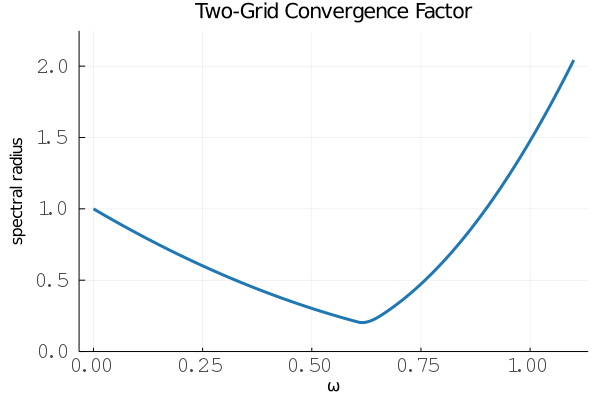
\includegraphics[width=0.48\textwidth]{../img/two_grid_converge_4_to_2}\label{fig:two_grid_4_2}}
    \subfloat[Convergence for $p = 4$ to $p = 1$, $\nu = 1$]{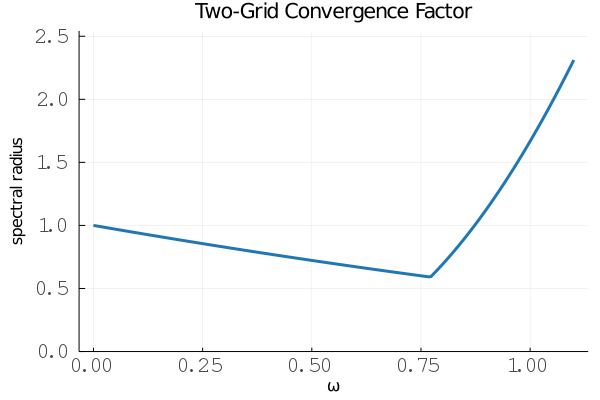
\includegraphics[width=0.48\textwidth]{../img/two_grid_converge_4_to_1}\label{fig:two_grid_4_1}} \\
    \subfloat[Convergence for $p = 4$ to $p = 2$, $\nu = 2$]{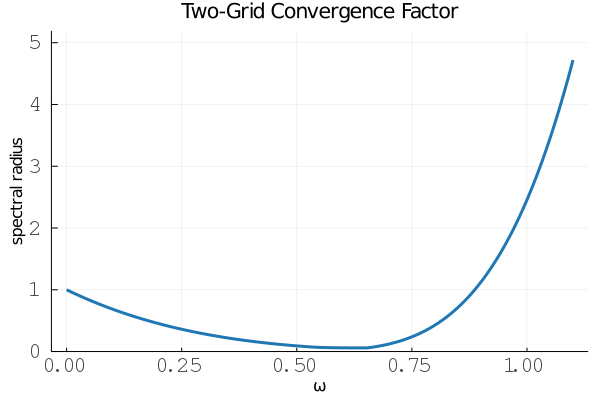
\includegraphics[width=0.48\textwidth]{../img/two_grid_converge_4_to_2_2smooth}\label{fig:two_grid_4_2_2smooth}}
    \subfloat[Convergence for $p = 4$ to $p = 1$, $\nu = 2$]{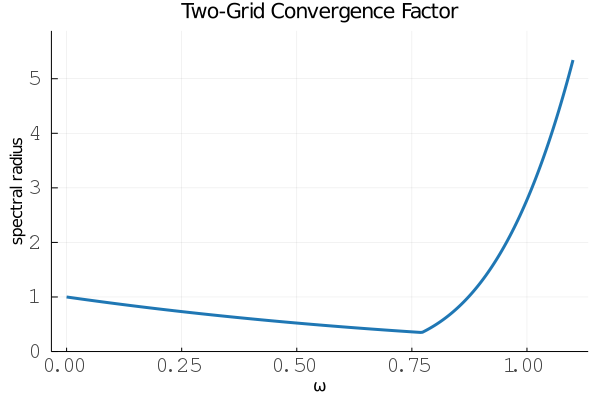
\includegraphics[width=0.48\textwidth]{../img/two_grid_converge_4_to_1_2smooth}\label{fig:two_grid_4_1_2smooth}} \\
  \caption{Two-grid analysis for Jacobi smoothing for high-order finite elements for the 1D Laplacian}
\end{figure}

In Figure \ref{fig:two_grid_4_2} and Figure \ref{fig:two_grid_4_1} we plot the two-grid convergence factor for $p$-multigrid with a single iteration of Jacobi pre and post-smoothing for the one dimensional Laplacian as a function of the Jacobi smoothing parameter $\omega$,
and in Figure \ref{fig:two_grid_4_2_2smooth} and Figure \ref{fig:two_grid_4_1_2smooth} we plot the two-grid convergence factor for $p$-multigrid with two iterations of Jacobi pre and post-smoothing for the one dimensional Laplacian as a function of the Jacobi smoothing parameter $\omega$.
On the left we show conservative coarsening from quartic to quadratic elements and on the right we show more aggressive coarsening from quartic to linear elements.
As expected, the two-grid convergence factor decreases as we coarsen more rapidly.
Also, the effect of underestimating the optimal Jacobi smoothing parameter, $\omega$, is less pronounced than the effect of overestimating the smoothing parameter, especially with a higher number of pre and post-smooths.

In contrast to the previous work on $h$-multigrid for high-order finite elements, \cite{he2020two}, poorly chosen values of $\omega < 1.0$ can result in a spectral radius of the $p$-multigrid error propagation symbol that is greater than $1$, indicating that application of $p$-multigrid with Jacobi smoothing at these parameter values will result in increased error.

\begin{table}[ht!]
\begin{center}
\begin{tabular}{l cc cc cc}
  \toprule
  $p_{\text{fine}}$ to $p_{\text{coarse}}$  &  \multicolumn{2}{c}{$\nu = 1$}  &  \multicolumn{2}{c}{$\nu = 2$}  &  \multicolumn{2}{c}{$\nu = 3$}  \\
  %\cmidrule(lr){2-3} \cmidrule(lr){4-5} \cmidrule(lr){6-7}
                       &  $\rho_{\min}$ & $\omega_{\text{opt}}$  &  $\rho_{\min}$ & $\omega_{\text{opt}}$  &  $\rho_{\min}$ & $\omega_{\text{opt}}$  \\
  \toprule
  $p = 2$ to $p = 1$   &  0.137 & 0.63  &  0.060 & 0.69  &  0.041 & 0.72   \\
  \midrule
  $p = 4$ to $p = 2$   &  0.204 & 0.62  &  0.059 & 0.64  &  0.045 & 0.70   \\
  $p = 4$ to $p = 1$   &  0.591 & 0.77  &  0.350 & 0.77  &  0.207 & 0.77   \\
  \midrule
  $p = 8$ to $p = 4$   &  0.250 & 0.60  &  0.068 & 0.60  &  0.033 & 0.63   \\
  $p = 8$ to $p = 2$   &  0.668 & 0.73  &  0.446 & 0.73  &  0.298 & 0.73   \\
  $p = 8$ to $p = 1$   &  0.874 & 0.78  &  0.764 & 0.78  &  0.668 & 0.78   \\
  \midrule
  $p = 16$ to $p = 8$  &  0.300 & 0.57  &  0.090 & 0.57  &  0.035 & 0.58   \\
  $p = 16$ to $p = 4$  &  0.719 & 0.69  &  0.517 & 0.69  &  0.371 & 0.69   \\
  $p = 16$ to $p = 2$  &  0.906 & 0.73  &  0.820 & 0.73  &  0.743 & 0.73   \\
  $p = 16$ to $p = 1$  &  0.968 & 0.74  &  0.936 & 0.74  &  0.906 & 0.74   \\
  \bottomrule
\end{tabular}
\end{center}
\caption{Two-grid convergence factor and optimal Jacobi parameter for the 1D Laplacian}
\label{table:two_grid_1d}
\end{table}

The results in Table \ref{table:two_grid_1d} provide the LFA convergence factor and optimal values of $\omega$ for two-grid high-order $p$-multigrid for a variety of polynomial orders and coarsening factors.

Traditional estimates of the optimal smoothing parameter based upon extremal eigevalues of the preconditioned operatro are incompatible with this LFA framework.
Optimal parameter estimation is an open question for high-order $p$-multigrid, but optimization techniques, such as those discussed in \cite{brown2021tuning}, can be used to tune these parameters, especially for more complex PDEs.

% -----------------------------------------------------------------------------
% Chebyshev Smoothing
% -----------------------------------------------------------------------------

\begin{figure}[!tbp]
  \centering
    \subfloat[Convergence for $p = 4$ to $p = 2$, $\nu = 1$]{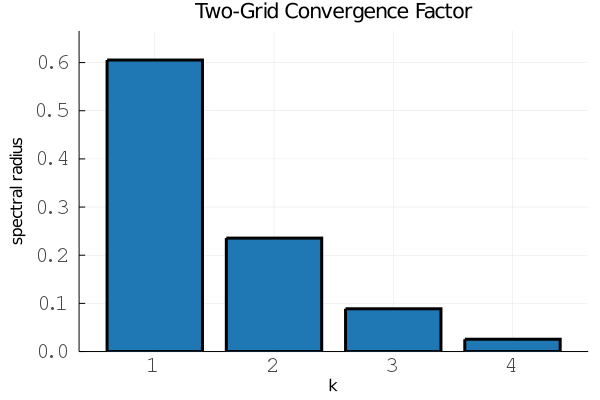
\includegraphics[width=0.48\textwidth]{../img/two_grid_converge_4_to_2_chebyshev}\label{fig:two_grid_4_2_chebyshev}}
    \subfloat[Convergence for $p = 4$ to $p = 1$, $\nu = 1$]{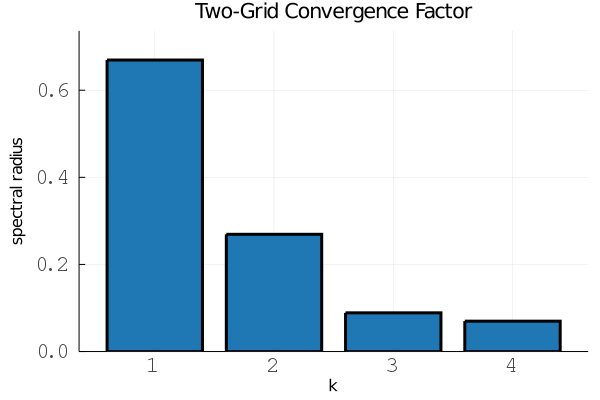
\includegraphics[width=0.48\textwidth]{../img/two_grid_converge_4_to_1_chebyshev}\label{fig:two_grid_4_1_chebyshev}}
  \caption{Two-grid analysis for Chebyshev smoothing for high-order finite elements for the 1D Laplacian}
\end{figure}

In Figure \ref{fig:two_grid_4_2_chebyshev} and Figure \ref{fig:two_grid_4_1_chebyshev} we plot the two-grid convergence factor for $p$-multigrid with Chebyshev pre and post-smoothing for the one dimensional Laplacian as a function of the Chebyshev order, $k$.
On the left we show conservative coarsening from quartic to quadratic elements and on the right we show more aggressive coarsening from quartic to linear elements.
As expected, the two-grid convergence factor decreases as we coarsen more rapidly.

\begin{table}[ht!]
\begin{center}
\begin{tabular}{l c c c c}
  \toprule
  $p_{\text{fine}}$ to $p_{\text{coarse}}$  &  $k = 1$   &  $k = 2$   &  $k = 3$   &  $k = 4$   \\
  %\cmidrule(lr){2-3} \cmidrule(lr){4-5} \cmidrule(lr){6-7}
  \toprule
  $p = 2$ to $p = 1$   &  0.545  &  0.220  &  0.063  &  0.017  \\
  \midrule
  $p = 4$ to $p = 2$   &  0.576  &  0.222  &  0.089  &  0.025  \\
  $p = 4$ to $p = 1$   &  0.623  &  0.269  &  0.089  &  0.070  \\
  \midrule
  $p = 8$ to $p = 4$   &  0.638  &  0.244  &  0.074  &  0.022  \\
  $p = 8$ to $p = 2$   &  0.657  &  0.260  &  0.097  &  0.059  \\
  $p = 8$ to $p = 1$   &  0.881  &  0.674  &  0.510  &  0.393  \\
  \midrule
  $p = 16$ to $p = 8$  &  0.664  &  0.253  &  0.075  &  0.022  \\
  $p = 16$ to $p = 4$  &  0.714  &  0.328  &  0.135  &  0.059  \\
  $p = 16$ to $p = 2$  &  0.907  &  0.741  &  0.602  &  0.496  \\
  $p = 16$ to $p = 1$  &  0.970  &  0.912  &  0.857  &  0.809  \\
  \bottomrule
\end{tabular}
\end{center}
\caption{Two-grid convergence factor with Chebyshev smoothing for 1D Laplacian}
\label{table:two_grid_1d_chebyshev}
\end{table}

The results in Table \ref{table:two_grid_1d_chebyshev} provide the LFA convergence factor and optimal values of $k$ for two-grid high-order $p$-multigrid for a variety of coarsening rates and orders of Chebyshev smoother.
From this table, we can see that the effectiveness of higher order Chebyshev smoothers degrades as we coarsen more aggressively, but Chebyshev smoothing still provides better two-grid convergence than multiple pre and post-smoothing Jacobi iterations.

\begin{table}[ht!]
\begin{center}
\begin{tabular}{l c c c c}
  \toprule
  \multicolumn{5}{c}{$\lambda_{\min} = 0.2 \hat{\lambda}_{\max}$} \\
  \toprule
  $p_{\text{fine}}$ to $p_{\text{coarse}}$  &  $k = 1$   &  $k = 2$   &  $k = 3$   &  $k = 4$   \\
  \toprule
  $p = 4$ to $p = 2$   &  0.410  &  0.093  &  0.043  &  0.024  \\
  $p = 4$ to $p = 1$   &  0.611  &  0.250  &  0.106  &  0.071  \\
  \midrule
  $p = 8$ to $p = 4$   &  0.435  &  0.081  &  0.016  &  0.007  \\
  $p = 8$ to $p = 1$   &  0.891  &  0.739  &  0.623  &  0.529  \\
  \midrule
  $p = 16$ to $p = 8$  &  0.443  &  0.081  &  0.015  &  0.006  \\
  $p = 16$ to $p = 1$  &  0.973  &  0.931  &  0.894  &  0.861  \\
  \toprule
  \multicolumn{5}{c}{$\lambda_{\min} = 0.3 \hat{\lambda}_{\max}$} \\
  \toprule
  $p_{\text{fine}}$ to $p_{\text{coarse}}$  &  $k = 1$   &  $k = 2$   &  $k = 3$   &  $k = 4$   \\
  \toprule
  $p = 4$ to $p = 2$   &  0.279  &  0.070  &  0.042  &  0.031  \\
  $p = 4$ to $p = 1$   &  0.638  &  0.332  &  0.184  &  0.104  \\
  \midrule
  $p = 8$ to $p = 4$   &  0.289  &  0.050  &  0.023  &  0.012  \\
  $p = 8$ to $p = 1$   &  0.899  &  0.777  &  0.682  &  0.599  \\
  \midrule
  $p = 16$ to $p = 8$  &  0.294  &  0.055  &  0.020  &  0.010  \\
  $p = 16$ to $p = 1$  &  0.975  &  0.942  &  0.913  &  0.885  \\
  \bottomrule
\end{tabular}
\end{center}
\caption{Two-grid convergence factor with Chebyshev smoothing for 1D Laplacian with modified lower eigenvalue bound.}
\label{table:two_grid_1d_chebyshev_eigenvalues}
\end{table}

The results in Table \ref{table:two_grid_1d_chebyshev_eigenvalues} provide the LFA-predicted convergence factor for two-grid high-order $p$-multigrid for a variety of coarsening rates and orders of Chebyshev smoother with different scaling factors for the minimum eigenvalue estimate used in the Chebyshev iterations.
Increasing the lower eigenvalue estimate results in the Chebyshev method better targeting high frequency error modes, which results in improved two-grid convergence when halving the polynomial degree of the basis functions.
However, increasing the lower eigenvalue estimate results in worse two-grid convergence for aggressive coarsening directly to linear elements.

% -----------------------------------------------------------------------------
\subsubsection{Scalar Laplacian - 2D Convergence Factors}\label{sec:2dresults}
% -----------------------------------------------------------------------------

% -----------------------------------------------------------------------------
% Jacobi Smoothing
% -----------------------------------------------------------------------------

In Figure \ref{fig:two_grid_converge_4_to_1_1_smooth_2d} and Figure \ref{fig:two_grid_converge_4_to_2_1_smooth_2d} we plot the two-grid convergence factor for $p$-multigrid with a single iteration of Jacobi pre and post-smoothing for the two dimensional Laplacian as a function of the Jacobi smoothing parameter $\omega$,
and in Figure \ref{fig:two_grid_converge_4_to_1_2_smooth_2d} and Figure \ref{fig:two_grid_converge_4_to_2_2_smooth_2d} we plot the two-grid convergence factor for $p$-multigrid with two iterations of Jacobi pre and post-smoothing for the two dimensional Laplacian as a function of the Jacobi smoothing parameter $\omega$.
On the left we show conservative coarsening from quartic to quadratic elements and on the right we show more aggressive coarsening from quartic to linear elements.
As we saw with one dimension, the two-grid convergence factor decreases as we coarsen more rapidly.
Also, the effect of underestimating the optimal Jacobi smoothing parameter, $\omega$, is less pronounced than the effect of overestimating the smoothing parameter, especially with a higher number of pre and post-smooths.

\begin{figure}[!tbp]
  \centering
  \subfloat[Convergence for $p = 4$ to $p = 2$, $\nu = 1$]{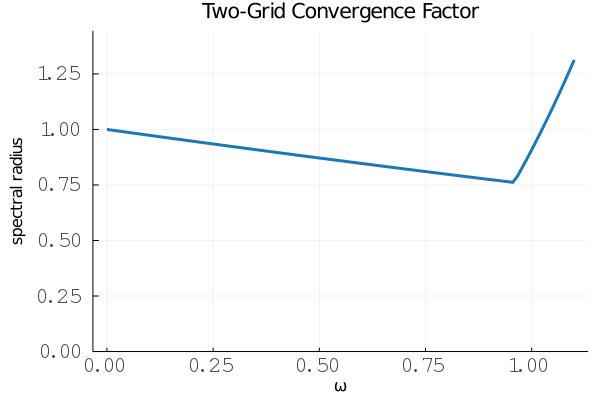
\includegraphics[width=0.48\textwidth]{../img/two_grid_converge_4_to_1_1_smooth_2d}\label{fig:two_grid_converge_4_to_2_1_smooth_2d}}
  \subfloat[Convergence for $p = 4$ to $p = 1$, $\nu = 1$]{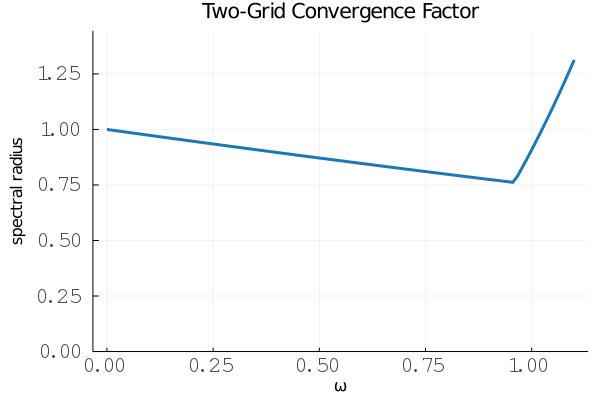
\includegraphics[width=0.48\textwidth]{../img/two_grid_converge_4_to_1_1_smooth_2d}\label{fig:two_grid_converge_4_to_1_1_smooth_2d}} \\
  \subfloat[Convergence for $p = 4$ to $p = 2$, $\nu = 2$]{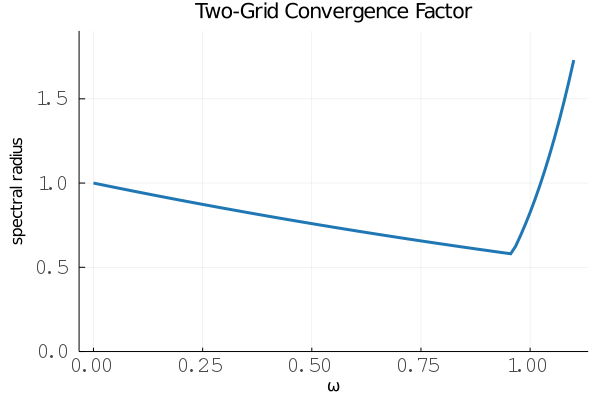
\includegraphics[width=0.48\textwidth]{../img/two_grid_converge_4_to_1_2_smooth_2d}\label{fig:two_grid_converge_4_to_2_2_smooth_2d}}
  \subfloat[Convergence for $p = 4$ to $p = 1$, $\nu = 2$]{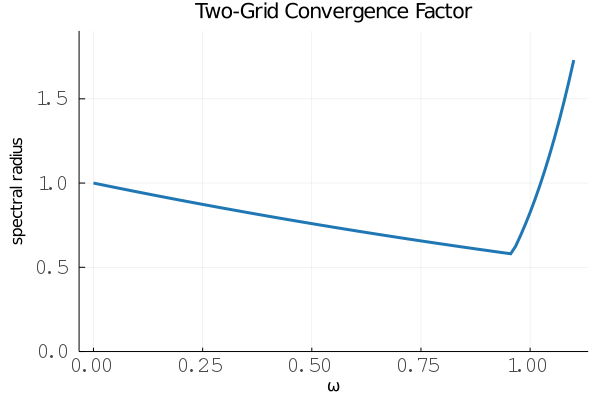
\includegraphics[width=0.48\textwidth]{../img/two_grid_converge_4_to_1_2_smooth_2d}\label{fig:two_grid_converge_4_to_1_2_smooth_2d}} \\
  \caption{Convergence for high-order finite elements for the 2D Laplacian}
\end{figure}

\begin{table}[ht!]
\begin{center}
\begin{tabular}{l cc cc cc}
  \toprule
  $p_{\text{fine}}$ to $p_{\text{coarse}}$  &  \multicolumn{2}{c}{$\nu = 1$}  &  \multicolumn{2}{c}{$\nu = 2$}  &  \multicolumn{2}{c}{$\nu = 3$}  \\
  %\cmidrule(lr){2-3} \cmidrule(lr){4-5} \cmidrule(lr){6-7}
                      &  $\rho_{\min}$  &  $\omega_{\text{opt}}$  &  $\rho_{\min}$ & $\omega_{\text{opt}}$  &  $\rho_{\min}$ & $\omega_{\text{opt}}$  \\
  \toprule
  $p = 2$ to $p = 1$  &  0.230 & 0.95  &  0.091 & 0.99  &  0.061 & 1.03   \\
  \midrule
  $p = 4$ to $p = 2$  &  0.388 & 0.82  &  0.151 & 0.82  &  0.078 & 0.83   \\
  $p = 4$ to $p = 1$  &  0.763 & 0.95  &  0.582 & 0.95  &  0.444 & 0.95   \\
  \midrule
  $p = 8$ to $p = 4$  &  0.646 & 0.79  &  0.418 & 0.79  &  0.272 & 0.79   \\
  $p = 8$ to $p = 2$  &  0.858 & 0.84  &  0.737 & 0.84  &  0.633 & 0.84   \\
  $p = 8$ to $p = 1$  &  0.952 & 0.87  &  0.907 & 0.87  &  0.864 & 0.87   \\
  \bottomrule
\end{tabular}
\end{center}
\caption{Two-grid convergence factor and optimal Jacobi parameter for 2D Laplacian}
\label{table:two_grid_2d}
\end{table}

The results in Table \ref{table:two_grid_2d} provide the LFA convergence factor and optimal values of $\omega$ for two-grid high-order $p$-multigrid for a variety of polynomial orders and coarsening factors.

% -----------------------------------------------------------------------------
% Chebyshev Smoothing
% -----------------------------------------------------------------------------

\begin{table}[ht!]
\begin{center}
\begin{tabular}{l c c c c}
  \toprule
  $p_{\text{fine}}$ to $p_{\text{coarse}}$  &  $k = 1$   &  $k = 2$   &  $k = 3$   &  $k = 4$   \\
  %\cmidrule(lr){2-3} \cmidrule(lr){4-5} \cmidrule(lr){6-7}
  \toprule
  $p = 2$ to $p = 1$   &  0.621  &  0.252  &  0.075  &  0.039  \\
  \midrule
  $p = 4$ to $p = 2$   &  0.607  &  0.281  &  0.085  &  0.047  \\
  $p = 4$ to $p = 1$   &  0.768  &  0.424  &  0.219  &  0.127  \\
  \midrule
  $p = 8$ to $p = 4$   &  0.669  &  0.278  &  0.110  &  0.055  \\
  $p = 8$ to $p = 2$   &  0.864  &  0.633  &  0.456  &  0.336  \\
  $p = 8$ to $p = 1$   &  0.956  &  0.873  &  0.795  &  0.730  \\
  \midrule
  $p = 16$ to $p = 8$  &  0.855  &  0.613  &  0.435  &  0.319  \\
  $p = 16$ to $p = 4$  &  0.938  &  0.822  &  0.719  &  0.634  \\
  $p = 16$ to $p = 2$  &  0.976  &  0.928  &  0.882  &  0.842  \\
  $p = 16$ to $p = 1$  &  0.992  &  0.975  &  0.959  &  0.944  \\
  \bottomrule
\end{tabular}
\end{center}
\caption{Two-grid convergence factor with Chebyshev smoothing for 2D Laplacian}
\label{table:two_grid_2d_chebyshev}
\end{table}

The results in Table \ref{table:two_grid_2d_chebyshev} provide the LFA convergence factor and optimal values of $k$ for two-grid high-order $p$-multigrid for a variety of coarsening rates and orders of Chebyshev smoother.
The two-grid convergence factor still degrades and the effectiveness of higher order Chebyshev smoothers is again reduced as we coarsen more aggressively.

\begin{table}[ht!]
\begin{center}
\begin{tabular}{l c c c c}
  \toprule
  \multicolumn{5}{c}{$\lambda_{\min} = 0.2 \hat{\lambda}_{\max}$} \\
  \toprule
  $p_{\text{fine}}$ to $p_{\text{coarse}}$  &  $k = 1$   &  $k = 2$   &  $k = 3$   &  $k = 4$   \\
  \toprule
  $p = 4$ to $p = 2$   &  0.450  &  0.137  &  0.067  &  0.050  \\
  $p = 4$ to $p = 1$   &  0.786  &  0.525  &  0.362  &  0.255  \\
  \midrule
  $p = 8$ to $p = 4$   &  0.668  &  0.330  &  0.172  &  0.106  \\
  $p = 8$ to $p = 1$   &  0.960  &  0.899  &  0.848  &  0.801  \\
  \toprule
  \multicolumn{5}{c}{$\lambda_{\min} = 0.3 \hat{\lambda}_{\max}$} \\
  \toprule
  $p_{\text{fine}}$ to $p_{\text{coarse}}$  &  $k = 1$   &  $k = 2$   &  $k = 3$   &  $k = 4$   \\
  \toprule
  $p = 4$ to $p = 2$   &  0.407  &  0.106  &  0.073  &  0.059  \\
  $p = 4$ to $p = 1$   &  0.803  &  0.590  &  0.447  &  0.341  \\
  \midrule
  $p = 8$ to $p = 4$   &  0.691  &  0.409  &  0.256  &  0.164  \\
  $p = 8$ to $p = 1$   &  0.963  &  0.915  &  0.874  &  0.835  \\
  \bottomrule
\end{tabular}
\end{center}
\caption{Two-grid convergence factor with Chebyshev smoothing for 2D Laplacian with modified lower eigenvalue bound.}
\label{table:two_grid_2d_chebyshev_eigenvalues}
\end{table}

The results in Table \ref{table:two_grid_2d_chebyshev_eigenvalues} provide the LFA-predicted convergence factor and optimal values of $k$ for two-grid high-order p-multigrid for a variety of coarsening rates and orders of Chebyshev smoother with different scaling factors for the minimum eigenvalue estimate used in the Chebyshev iterations.
As in one dimension, increasing the lower eigenvalue estimate results in better two-grid convergence when conventional coarsening by halving the polynomial degree of the basis functions but results in worse two-grid convergence with aggressive coarsening.

% -----------------------------------------------------------------------------
\subsubsection{Linear Elasticity - 3D Convergence Factors}\label{sec:solidsresults}
% -----------------------------------------------------------------------------

To demonstrate the suitability of this LFA formulation for more complex PDE, we consider linear elasticity in three dimensions.
The strong form of the static balance of linear momentum at small strain for the three dimensional linear elasticity problem is given by \cite{hughes2012finite} as
\begin{equation}
\nabla \cdot \boldsymbol{\sigma} + \boldsymbol{g} = \boldsymbol{0}
\end{equation}
where $\boldsymbol{\sigma}$ is the stress function and $\boldsymbol{g}$ is the forcing function.
This strong form has the corresponding weak form
\begin{equation}
\int_{\Omega} \nabla \mathbf{v} : \boldsymbol{\sigma} dV - \int_{\partial \Omega} \mathbf{v} \cdot \left( \boldsymbol{\sigma} \cdot \hat{\mathbf{n}} \right) dS - \int_{\Omega} \mathbf{v} \cdot \mathbf{g} dV = 0, \forall \mathbf{v} \in \mathcal{V}
\end{equation}
for some displacement $\mathbf{u} \in \mathcal{V} \subset H^1 \left( \Omega \right)$, where $:$ denotes contraction over both components and dimensions.

Linear elasticity constitutive modeling is based upon the Lamé parameters,
\begin{equation}
\begin{split}
\lambda & = \frac{E \nu}{\left( 1 + \nu \right) \left( 1 - 2 \nu \right)} \\
\mu & = \frac{E}{2 \left( 1 + \nu \right)}
\end{split}
\end{equation}
where $E$ is the Young's modulus and $\nu$ is the Poisson's ratio for the materiel.

In the linear elasticity constitutive model, the symmetric strain tensor is given by
\begin{equation}
\boldsymbol{\epsilon} = \frac{1}{2} \left( \nabla \mathbf{u} + \nabla \mathbf{u}^T \right)
\end{equation}
and the linear elasticity constitutive law is given by $\boldsymbol{\sigma} = \mathsf{C} : \boldsymbol{\epsilon}$ where
\begin{equation}
\mathsf{C} =
\begin{bmatrix}
   \lambda + 2\mu & \lambda & \lambda & & & \\
   \lambda & \lambda + 2\mu & \lambda & & & \\
   \lambda & \lambda & \lambda + 2\mu & & & \\
   & & & \mu & & \\
   & & & & \mu & \\
   & & & & & \mu
\end{bmatrix}.
\end{equation}

\begin{table}[ht!]
\begin{center}
\begin{tabular}{l c c c c}
  \toprule
  $p_{\text{fine}}$ to $p_{\text{coarse}}$  &  $k = 1$   &  $k = 2$   &  $k = 3$   &  $k = 4$   \\
  %\cmidrule(lr){2-3} \cmidrule(lr){4-5} \cmidrule(lr){6-7}
  \toprule
  $p = 2$ to $p = 1$   &  0.621  &  0.252  &  0.075  &  0.039  \\
  \midrule
  $p = 4$ to $p = 2$   &  0.607  &  0.281  &  0.085  &  0.047  \\
  $p = 4$ to $p = 1$   &  0.768  &  0.424  &  0.219  &  0.127  \\
  \midrule
  $p = 8$ to $p = 4$   &  0.669  &  0.278  &  0.110  &  0.055  \\
  $p = 8$ to $p = 2$   &  0.864  &  0.633  &  0.456  &  0.336  \\
  $p = 8$ to $p = 1$   &  0.956  &  0.873  &  0.795  &  0.730  \\
  \bottomrule
\end{tabular}
\end{center}
\caption{Two-grid convergence factor with Chebyshev smoothing for 3D linear elasticity}
\label{table:two_grid_3d_linear_elasticity}
\end{table}

The results in Table \ref{table:two_grid_3d_linear_elasticity} provide the LFA convergence factor and optimal values of $k$ for two-grid high-order $p$-multigrid for a variety of coarsening rates and orders of Chebyshev smoother.
